% witness: 2410.06985 (a structure diagram's blank node `\node[…]{\phantom{Cpd}\\\phantom{pt}}`; CL162)
% oracle:  pdflatex 0 errors: both nodes the same size, the first blank; Perl lists the node text's open-brace box in
%          the paragraph (TeX_Box.pool.ltxml:30-42), so the `\\` keeps the Cpd phantom (Stomach.pm:463-465)
% engines: rust int162a = the first node holds only <p><text class="ltx_phantom">pt</text></p>; Cpd lost
% expect:  0 errors, 0 warnings; the first node's phantoms Cpd and pt, the second node's text Cpd and pt
% status:  RED (int162a) -> GREEN (RG1)
\documentclass{article}
\usepackage{tikz}
\begin{document}
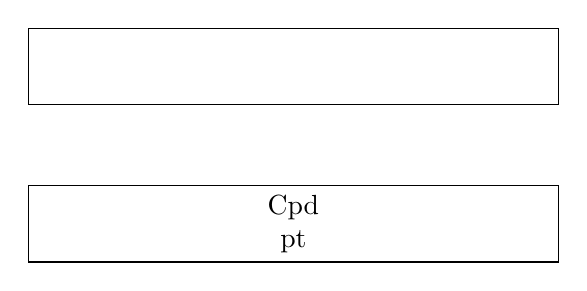
\begin{tikzpicture}
\node[draw, text width=6.5cm, align=center] {\phantom{Cpd}\\\phantom{pt}};
\node[draw, text width=6.5cm, align=center] at (0,-2) {Cpd\\pt};
\end{tikzpicture}
\end{document}
